\section{Accidental Background}\label{section:star_accidentals}
The accidental backgrounds (same bunch pile-up background) are quantified using data-driven method and defined as a process where in  single bunch crossing there is coincidence of two interactions, where any single-side proton signal is collected in coincidence with a~signal in the~TPC-TOF detector. %This has the same signature as a signal process but would not come from a DD, a CD or a ND interaction. 
This type of background may come from the overlap of a~signal in \ac{RP} (proton from beamhalo, low mass \ac{SD} process without activity in TOF, elastic or low mass \ac{CD} processes with undetected proton on the other side) with a~signal in TPC+TOF (mainly \ac{ND} events without forward proton).

The accidental background contribution was calculated  from Zerobias data, where two signatures of such background were investigated: the reconstructed proton in RP and the reconstruction of vertex from TPC tracks matched with TOF. The analysis was done for each RP arm separately and thus the 
 Zerobias data was firstly required to pass the following criteria:
\begin{enumerate}
	\item no trigger in any RP or trigger in exactly one arm (two RPs) with exactly one reconstructed proton track in that arm,
	\item veto on any signal in small BBC tiles or ZDC on the same  side of the IP as  RP under consideration,
	\item no or exactly one reconstructed vertex with at least two TOF-matched tracks passing the quality criteria. The latter includes also signal in BBC small tiles on the opposite side of the IP to the RP under study. 
\end{enumerate}
 The sample of selected Zerobias data with total  number  of events $N$ was divided into four classes:
\begin{equation}
N=N(P,S)+N(R,S)+N(P,T)+N(R,T)
\label{eq:accidentalSTAR_N}
\end{equation}
where: $N(P,S)$ is the~number of events with reconstructed proton in exactly one RP and reconstructed TOF vertex, $N(R,S)$  is the~number of events with no trigger in any RP and reconstructed TOF vertex, $N(P,T)$ is the~number of events with reconstructed proton in exactly one RP and no reconstructed TOF vertex, $N(R,T)$ is the~number of events with no trigger in any RP and no reconstructed TOF vertex.\\

Since the signature of the signal is a reconstructed proton in exactly one RP and a~reconstructed TOF vertex, the number of such events can be expressed as:
\begin{equation}
N(P,S)=N\left(p_3+p_1p_2\right)
\end{equation}
where: $p_1$ is the~probability that there is a~reconstructed proton in RP and there is no reconstructed TOF vertex, $p_2$ is the~probability that there is no reconstructed proton in RP and  there is a~reconstructed TOF vertex, $p_3$ is the~probability that there is a~reconstructed proton in RP and  there is a~reconstructed TOF vertex (not accidental).

The other classes of events given in Eq.~\eqref{eq:accidentalSTAR_N} can be expressed in terms of the~above probabilities as:
\begin{equation}
\begin{split}
N(R,S)=  & N(1-p_1)p_2(1-p_3)\\
N(P,T) = & N(1-p_2)p_1(1-p_3)\\
N(R,T) = & N(1-p_1)(1-p_2)(1-p_3)
\end{split}
\end{equation}
Finally, the accidental background contribution $A_{\mathrm{bkg} }^{\mathrm{accidental}}$ is  given by:
\begin{equation}
\begin{split}
A_{\mathrm{bkg}}^{\mathrm{accidental}}=  \frac{p_1p_2}{p_3+p_1p_2}=\frac{N(R,S)N(P,T)N}{N(R)N(T)N(P,S)}
\end{split}
\label{eq:bkg_acc_norm}
\end{equation} 
where: $N(R)=N(R,S)+N(R,T)$ and $N(T)=N(P,T)+N(R,T)$.

The shapes of the accidental background related to TPC distributions come from the~above Zerobias data events which pass all the analysis selection except having no trigger in any RP. The~templates corresponding to RP distributions are from protons in the~above data sets but with no reconstructed TOF vertex. The normalization is given by Eq.~\eqref{eq:bkg_acc_norm}. Figure~\ref{fig:STARaccidentalsXi} shows distributions of the~reconstructed $\xi$ with the~accidental background contribution  for events with proton reconstructed in EU, ED, WU and WD arms. Accidental background in the~range of $0.02<\xi<0.2$ is below $1\%$.

\begin{figure}[h!]
	\centering
	\includegraphics[width=0.49\textwidth, page=40]{chapters/chrgSTAR/img/accidentals/accidentalBkg.pdf}
	\includegraphics[width=0.49\textwidth, page=41]{chapters/chrgSTAR/img/accidentals/accidentalBkg.pdf}
	\includegraphics[width=0.49\textwidth, page=42]{chapters/chrgSTAR/img/accidentals/accidentalBkg.pdf}
	\includegraphics[width=0.49\textwidth, page=43]{chapters/chrgSTAR/img/accidentals/accidentalBkg.pdf}
	\caption{Uncorrected distributions of the reconstructed $\xi$ for events with proton reconstructed in  (top left) EU, (top right) ED, (bottom left) WU and (bottom right) WD arms. Data is shown as black markers, whereas the~accidental background contribution is shown as yellow histogram.  The ratio of accidental background and data is shown in the bottom pad.}
	\label{fig:STARaccidentalsXi}
\end{figure}

The selection of Zerobias events, which is not unique, may provide some bias to the normalization of the~accidental background. As a systematic check, two criteria for  Zerobias selection were changed~to:
 \begin{enumerate}
 	\item no trigger in any RP or trigger in exactly one arm (two RPs) with \textit{no more} than one reconstructed proton track in that arm, i.e. events with trigger signals in exactly one arm and without reconstructed proton track in that arm were also used,
 	%\item veto on any signal in small BBC tiles or ZDC on the same  side of the IP as  RP under study,
 	\item no  or exactly one reconstructed TOF vertex (%not necessarily  with two TOF-matched tracks passing the quality criteria). 
 	\textit{without any additional requirements}), i.e. events with a~reconstructed TOF vertex that does not have at least two primary tracks satisfying the~selection criteria (Sec.~\ref{section:star_track_selection}), or with a~reconstructed TOF vertex that is out of the~range of $|V_z|<80$~cm, were also accepted. The requirement of signal in BBC small tiles remains unchanged. 
 \end{enumerate}
 As a result of this change in the procedure%, as shown in Fig.~\ref{fig:STARaccidentalsXiSyst}, 
 the accidental background normalization increases of about $50\%$ with respect to the nominal value. Therefore, the background changes by $\pm50\%$ was taken as a systematic uncertainty related to the accidentals.
 
 \begin{comment}
 \begin{figure}[h!]
 	\centering
 	\includegraphics[width=0.49\textwidth, page=40]{chapters/chrgSTAR/img/accidentals/accidentalBkg_test.pdf}
 	\includegraphics[width=0.49\textwidth, page=41]{chapters/chrgSTAR/img/accidentals/accidentalBkg_test.pdf}
 	\includegraphics[width=0.49\textwidth, page=42]{chapters/chrgSTAR/img/accidentals/accidentalBkg_test.pdf}
 	\includegraphics[width=0.49\textwidth, page=43]{chapters/chrgSTAR/img/accidentals/accidentalBkg_test.pdf}
 	\caption{Uncorrected distributions of the reconstructed $\xi$ for events with proton reconstructed in (top left) EU, (top right) ED, (bottom left) WU and (bottom right) WD arms. The~accidental background contribution calculated with changed Zerobias selection criteria is also shown.}
 	\label{fig:STARaccidentalsXiSyst}
 \end{figure}
\end{comment}



